\chapter{Tutorials}

%%%%%%%%%%%%%%%%%%%%%%%%%%%%%%%%%%%%%%%%%%%%%%%%%%%%%%%%%%%%%%%%%%%%%%%%%%%%%%
\section{Using AlphaFlow in a default Plone installation}
%%%%%%%%%%%%%%%%%%%%%%%%%%%%%%%%%%%%%%%%%%%%%%%%%%%%%%%%%%%%%%%%%%%%%%%%%%%%%%

AlphaFlow can be used as a drop-in replacement for Plone's own workflow
mechanism and comes with a few pre-defined workflows. One of those implements
the same kind of reviews as the standard Plone workflow.

This tutorial assumes that you use a Plone 2.5 portal with AlphaFlow installed
and the default content types patched to support AlphaFlow.

%%%%%%%%%%%%%%%%%%%%%%%%%%%%%%%%%%%%%%%%%%%%%%%%%%%%%%%%%%%%%%%%%%%%%%%%%%%%%%
\subsection{Selecting a workflow}

First we need to add a new content object that we want to run a workflow for:
\begin{itemize}
\item Add a new document to your portal. Make sure you saved it once.
\item There is now a new object action called ``select workflow''.
\item The old workflow menu now only displays the status and is ``visible'' in the beginning.
\end{itemize}

Now we can start using a workflow:
\begin{itemize}
\item Click on the ``Select workflow'' action. It will display a list of available workflows.
\item On the workflow listing, you get an overview chart by clicking on the workflow
    icon next to each workflow's title. Here is the chart for the ``simple review'':
\begin{figure}
  \centering
  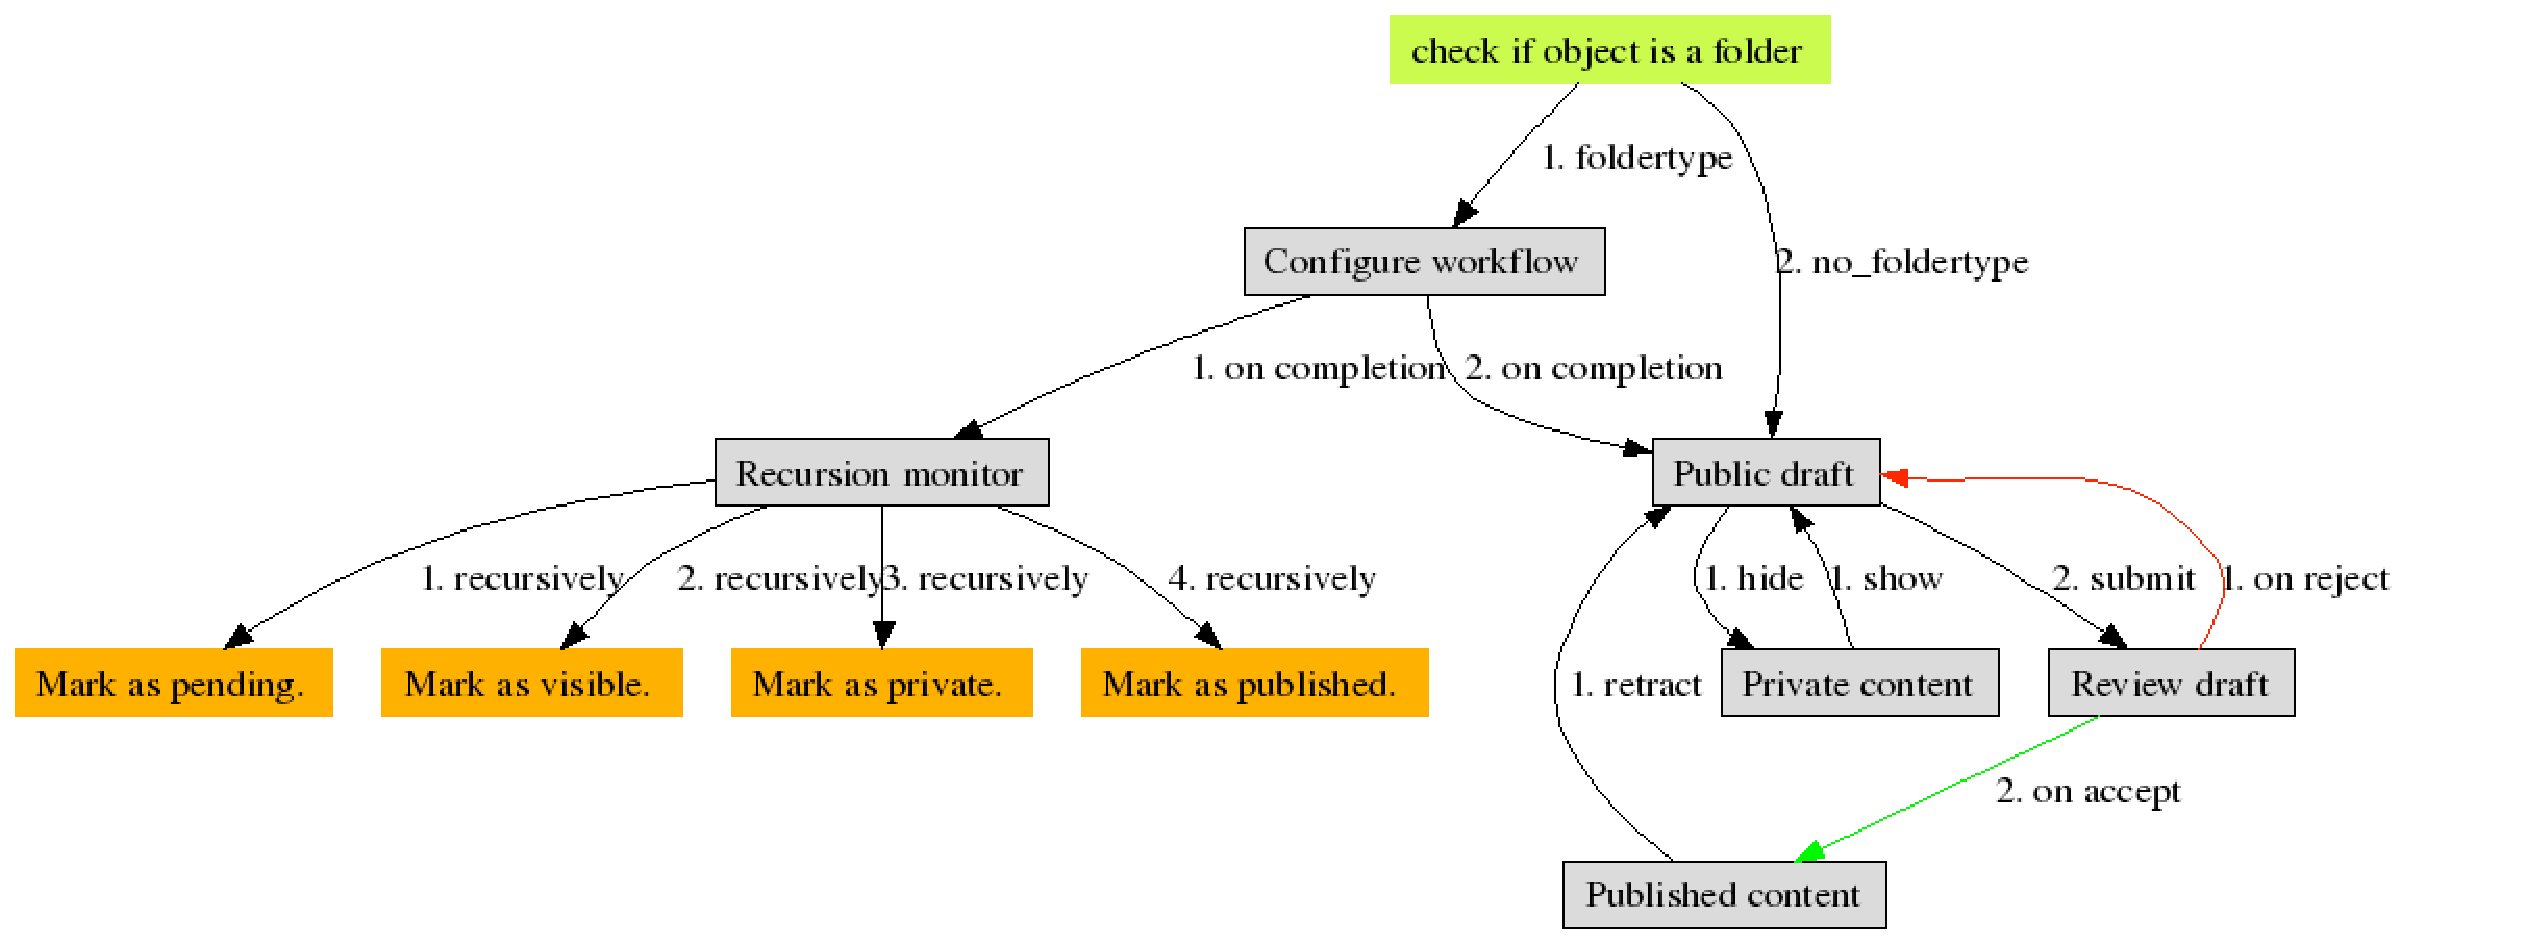
\includegraphics[width=19cm]{simplereview}
  \caption{\label{fig:simplereview}%
    Simple review}
\end{figure}
\item Now, click on the title ``simple review'' to select this workflow for the document.
\item Plone responds with a status message telling you that the workflow has been started.
\end{itemize}

%%%%%%%%%%%%%%%%%%%%%%%%%%%%%%%%%%%%%%%%%%%%%%%%%%%%%%%%%%%%%%%%%%%%%%%%%%%%%%
\subsection{Workflow menu}

After selecting a workflow, the ``workflow menu'' allows everybody involved
with a workflow to perform various operations:

\begin{itemize}
\item Open the workflow menu.
\end{itemize}

The upper part of the menu is titled ``public draft'' followed by three
actions.  You can use the menu to either edit your document in private, submit
it for review or stop the workflow.

In other workflows this menu will have different entries depending on the
actual activities in the workflow.

%%%%%%%%%%%%%%%%%%%%%%%%%%%%%%%%%%%%%%%%%%%%%%%%%%%%%%%%%%%%%%%%%%%%%%%%%%%%%%
\subsection{The work list portlet (``my tasks'')}

When you started the workflow a work item was assigned to you, asking you to
edit the document.  Whenever you have a work item assigned, the portlet ``my
tasks'' will appear and inform you about work items assigned to you. It now
contains the ``write document'' task.

\begin{itemize}
\item Go to the portal home page and follow the link in the work item.
\end{itemize}

You are now back at the document you started the workflow on. The work list
will link you to a relevant page for the work item. In many cases this will be
the content object.

\begin{itemize}
\item Create a new document and also start a ``simple review'' workflow on it.
\end{itemize}

The task portlet has two entries now: one ``public draft'' work item for each
document.

\begin{itemize}
\item Look at the workflow menu of both documents.
\end{itemize}

Both still have only one entry. While the worklist portlet collects all work
items assigned to you on any portal objects, the workflow menu refers to the
work items of the current content object only.

%%%%%%%%%%%%%%%%%%%%%%%%%%%%%%%%%%%%%%%%%%%%%%%%%%%%%%%%%%%%%%%%%%%%%%%%%%%%%%
\subsection{Completing the task}

The workflow menu offers you a list of actions for the ``public draft'' work item. Lets hide the document while we are editing it:

\begin{itemize}
    \item Select the ``hide'' action from the workflow menu.
    \item Enter a comment why we are hiding the document.
    \item Let the action remain on the setting ``hide''.
    \item Click ``submit'' to perform the action.
\end{itemize}

When the work item was completed using the ``hide'' action, the ``simple review'' performed several things:
\begin{itemize}
    \item The workflow status has now changed to ``private''.
    \item The workflow menu now contains a different work item. It is called ``private content''. 
    \item The work list now displays the ``private content'' work item instead of ``edit document.
\end{itemize}

%%%%%%%%%%%%%%%%%%%%%%%%%%%%%%%%%%%%%%%%%%%%%%%%%%%%%%%%%%%%%%%%%%%%%%%%%%%%%%
\subsection{Workflow details}
\label{sec:tut-details}

Now that some things have happened in the workflow, lets look at
the detailed workflow overview.

\begin{itemize}
\item Choose the ``details'' action in the workflow menu of the document you hid
  in the previous step.
\end{itemize}

The details view shows various information:

\begin{itemize}
\item There are two lists of work items, one listing all work items currently
  running, the other reporting on work items already completed. Both show work
  item titles and descriptions and some administrative data.
\item The current list contains one entry for the ``private content'' work
  item which also appears in the workflow menu and the portlet.
\item The history list contains the work item you completed, showing the
  comment you entered for it.
\item The history also lists some work items that were
  run without your interaction when the work flow was started and when you had
  completed the ``public draft'' work item. It is some of those automatic work
  items that updated the DCWorkflow state, others set the permissions on the
  content object as appropriate for making it a public draft or hiding it.
\end{itemize}

%%%%%%%%%%%%%%%%%%%%%%%%%%%%%%%%%%%%%%%%%%%%%%%%%%%%%%%%%%%%%%%%%%%%%%%%%%%%%%
\subsection{Recursive publication of folders}

Working with the rest of the workflow is similar to the first activity. You can
now submit, review and publish it. 

There is another feature of the ``simple review'' workflow worth examining more
closely, though: recursive folder publication and the configuration thereof.

\begin{itemize}
\item Create a new folder in your portal, create some documents and folders
  inside it, and start a ``simple review'' workflow on the folder.
\item A configuration form is displayed.
\item Select the given option for ``recursive publication''
\item Do a series of workflow actions on the folder: hide, show, submit. After
  each, look at objects inside the folder.
\item Notice how the DCWorkflow status displayed is always kept up-to-date
  with the status of the folder itself.
\item Notice also that there is no workflow running on the folder's documents
  and sub-folders. The workflow on the containing folder now affects all
  content objects inside it as well.
\end{itemize}

%%%%%%%%%%%%%%%%%%%%%%%%%%%%%%%%%%%%%%%%%%%%%%%%%%%%%%%%%%%%%%%%%%%%%%%%%%%%%%
\section{Developing an AlphaFlow application}
%%%%%%%%%%%%%%%%%%%%%%%%%%%%%%%%%%%%%%%%%%%%%%%%%%%%%%%%%%%%%%%%%%%%%%%%%%%%%%

Let us introduce AlphaFlow by writing an example application: a procurement
request system. A procurement request system allows you to manage
requests for buying things at your office.
    
On the user's side, some information needs to be entered for each request.
This includes a description of the item to buy, its price, the date it should
be bought, and the relevant account number for your accounting. More data
might be interesting for large scale applications, but this is enough to get a
useful application running.

However, each office using this system will have different rules on who has to
review the request, who is going to buy it, what happens if the request is
rejected, and so on.

This kind of flexibility is made possible by a workflow engine. It adds a
high-level flow control mechanism and allows you to customize the application
to your needs without modifying the application code itself.

\begin{notice}
  All code examples in this tutorial are taken from the code of the example
  application. It can be found in the
  \file{AlphaFlow/doc/examples/Procurement/} directory.
\end{notice}

%%%%%%%%%%%%%%%%%%%%%%%%%%%%%%%%%%%%%%%%%%%%%%%%%%%%%%%%%%%%%%%%%%%%%%%%%%%%%%
% \subsection{TODO A look at the demo application}

%%%%%%%%%%%%%%%%%%%%%%%%%%%%%%%%%%%%%%%%%%%%%%%%%%%%%%%%%%%%%%%%%%%%%%%%%%%%%%
\subsection{Application layout}

The procurement request system is a simple Archetypes application. It provides
two classes which are defined in \file{Procurement/request.py}:
\begin{description}
\item[\class{ProcurementRequest}] an Archetypes object storing the data of
  one procurement request
\item[\class{RequestManager}] an Archetypes folder storing procurement
  requests and providing access to various listings of requests
\end{description}

Procurement requests shall be governed by an AlphaFlow workflow. Therefore,
the \class{ProcurementRequest} class must be AlphaFlow-aware:
\begin{enumerate}
\item The first base class must be \class{AlphaFlowed}:

\begin{verbatim}
class ProcurementRequest(Products.AlphaFlow.public.AlphaFlowed, 
                         Products.Archetypes.public.BaseContent):
\end{verbatim}

\item \class{ProcurementRequest} has to declare that it implements the same
  interfaces as \class{AlphaFlowed} along with the interfaces of the other
  base classes:

\begin{verbatim}
    __implements__ = Products.AlphaFlow.public.AlphaFlowed.__implements__ + \
                     Products.Archetypes.public.BaseContent.__implements__
\end{verbatim}
\end{enumerate}

AlphaFlow allows the application to decide when a workflow is connected with a
content object, and which workflow that is. In our case, each
\class{ProcurementRequest} object is assigned a workflow named
``procurement'' and the instance is run immediately.
    
\begin{verbatim}
    def manage_afterAdd(self, item, container):
        Request.inheritedAttribute('manage_afterAdd')(self, item, container)

        self.assignProcess("procurement")
        self.getInstance().start("Workflow started by request creation.")
\end{verbatim}

\begin{notice}
  The code examples use a more verbose form of referencing class names than is
  used in the actual product code. E.g.
  \class{Products.AlphaFlow.public.AlphaFlowed} will usually be written as
  \class{afapi.AlphaFlowed} in the example product, the AlphaFlow public API
  being imported:
\begin{verbatim}
from Products.AlphaFlow import public as afapi
\end{verbatim}
\end{notice}

In the next step we will define and import a workflow definition.
    
%%%%%%%%%%%%%%%%%%%%%%%%%%%%%%%%%%%%%%%%%%%%%%%%%%%%%%%%%%%%%%%%%%%%%%%%%%%%%%
\subsection{Defining the workflow}

Now we construct a workflow which will handle procurement requests. We will
start with a simple process and evolve it to a more complex setup, introducing
several AlphaFlow features along the way.

\subsubsection{An empty workflow definition}

Workflow definitions are written in an XML syntax called ALF. The XML
definition of the workflow governing our procurement requests starts out like
this:

\begin{verbatim}
<?xml version="1.0" encoding="utf-8"?>

<workflow id="procurement"
          title="Simple Procurement"
          description=
    "A procurement is requested, decided upon and possibly carried out.">

</workflow>
\end{verbatim}

Some comments about the anatomy of this file:
\begin{enumerate}
\item The root element of every ALF file is \member{workflow}.
\item To suggest an id for this workflow definition, the \member{id} attribute
  can be set.
\item The attributes \member{title} and \member{description} characterize
  each process in the user interface.
\end{enumerate}
            
\subsubsection{Adding an activity}

AlphaFlow knows several kinds of activities for describing different steps of
a workflow. We represent the task of writing a procurement request by the
\member{task} activity. Tasks can be assigned to users. After a user has
completed a task, more activities are started. Our workflow definition now
reads:

\begin{verbatim}
<workflow id="procurement"
          ...
          startActivity="edit">

  <task id="edit"
        title="Edit a procurement request"
        completion_activity="review">

    <assignees kind="actual"
               expression="python:[request.Creator()]" />
  </task>

</workflow>
\end{verbatim}

Notes:
\begin{enumerate}
\item The attribute \member{startActivity} of the \member{workflow} element
  lists activities that are started at the beginning of the workflow.
\item Every activity must have an \member{id} so it can be referenced within
  the workflow definition, e.g. as a starting activity.
\item If a \member{title} is given, it appears in the user interface.
\item \member{completion\_activity} lists the activities to be started after
  the user has completed the task. The \member{review} activity will be added
  in the next step of the tutorial.
\item Users are assigned a task by adding the \member{assignees} element to
  the workflow definition. We select the creator of the procurement request by
  specifying a TALES expression.
\end{enumerate}

\subsubsection{Completing the workflow model}

Our workflow involves two more steps: deciding upon the procurement request
made, and buying the item if the request was accepted. The decision whether or not to buy the
requested item requires an activity that supports more than one outcome. 
The \member{decision} activity suits this best:

\begin{verbatim}
  <decision id="review"
            title="Decide whether the article should be bought."
            accept_activity="buy"
            reject_activity=""
            decision_modus="first_yes">

    <assignees kind="actual"
               roles="Finance" />
  </decision>

  <task id="buy"
        title="Buy">

    <assignees kind="actual"
               roles="Procurement" />
  </task>
\end{verbatim}

Notes:
\begin{enumerate}
\item The \member{decision} activity continues with either the activities
  listed in the \member{accept\_activity}, or those listed in the
  \member{reject\_activity} attribute.
\item A decision can be based on input from multiple users. The
  \member{decision_modus} ``first_yes'' means that the request will be
  accepted as soon as any assigned user accepts it.
\item Assignees can be chosen not only by listing their IDs in a TALES
  expressions, but also by giving one or more roles. In that case, all users
  with any of the listed roles are assigned the activity.
\item A workflow can include steps that are not performed within Plone,
  but in other systems or the real world. After the assigned user has bought
  the item, he declares the task ``buy'' completed.
\end{enumerate}

\subsubsection{Emulating DCWorkflow states}

AlphaFlow replaces Plone's own workflow engine, DCWorkflow. It does, however,
not remove it completely. Rather, AlphaFlow uses the fact that DCWorkflow's
states are well integrated with Plone to easily provide the user with
additional information on the progress of workflow instances.

A DCWorkflow state is a label attached to the content object of a given
workflow instance. It is set by the \member{dcworkflow} activity. In our
example, it makes sense to update the DCWorkflow state on completion of each
step in the workflow:

\begin{verbatim}
  <task id="edit"
        ...
        startActivity="dc_private">

  <decision id="review"
            ...
            startActivity="dc_pending"
            reject_activity="dc_rejected">

  <task id="buy"
        ...
        startActivity="dc_accepted"
        completion_activity="dc_bought">

  <dcworkflow id="dc_private"
              title="Mark as private."
              status="private" />

  <dcworkflow id="dc_pending"
              title="Mark as pending"
              status="pending" />

  <dcworkflow id="dc_accepted"
              title="Mark as accepted."
              status="accepted" />

  <dcworkflow id="dc_bought"
              title="Mark as bought."
              status="bought" />

  <dcworkflow id="dc_rejected"
              title="Mark as rejected."
              status="rejected" />
\end{verbatim}

Notes:
\begin{enumerate}
\item The \member{dcworkflow} activity is not assigned to any users. A
  \member{dcworkflow} work item is run automatically as soon as it is created,
  and finishes without waiting for user interaction.
\item The attribute \member{status} is the label to be attached to the content
  object. It may be any string.
\item There are some DCWorkflow states that have special meaning to Plone.
  Among them are ``private'' and ``pending''.
\end{enumerate}

Look at \file{AlphaFlow/doc/examples/Procurement/workflows/minimal.alf} to see
what the final version of the process definition looks like.

%%%%%%%%%%%%%%%%%%%%%%%%%%%%%%%%%%%%%%%%%%%%%%%%%%%%%%%%%%%%%%%%%%%%%%%%%%%%%%
\subsection{Extending the workflow}

In the previous sections of this tutorial, we constructed a procurement
request manager that subjects each request to a straight three-part workflow:
After a request has been created, it is edited by its creator and reviewed by
a user responsible for finance. If the request is accepted, the requested item
is bought by a user doing procurement.

\subsubsection{Adding an editing cycle}

Let's now add some more functionality to this minimal workflow. We want to
enable the reviewer to return the request to its creator for further editing
in addition to accepting and rejecting it for good.

We replace the ``review'' activity like this:

\begin{verbatim}
  <ntask id="review"
         title="Decide whether the article should be bought."
         startActivity="dc_pending">

    <assignees kind="actual"
               roles="Finance" />

    <exit id="accept"
          title="Accept"
          activities="buy" />

    <exit id="reject"
          title="Reject"
          activities="dc_rejected" />

    <exit id="return"
          title="Return for editing"
          activities="edit" />
  </ntask>
\end{verbatim}

Notes:
\begin{enumerate}
\item The \member{decision} activity supports only decisions that yield
  one of two possible results. A more general activity allowing for any number
  of ways to complete a task is \member{ntask}.
\item A user who completes an \member{ntask} has to choose an \member{exit} to
  take. The \member{id} and \member{title} of an exit serve to present the
  user with his choices and determine the exit he selects.
\item When an \member{ntask} is completed, only those activities listed in the
  \member{activities} attribute of the exit taken are started.
\end{enumerate}

You can find the complete workflow as extended in this section in
\file{AlphaFlow/doc/examples/Procurement/workflows/simple.alf}.

\subsubsection{Adding account-based review}

Suppose your book-keeping distinguishes multiple accounts for buying different
kinds of things. We will extend the review workflow such that a second person
has to agree to the request in addition to the financial supervisor. That
person is chosen depending on the account the requested item is booked on.

Combining the results of separate activities, which may, e.g., be assigned to
different users, requires routing the workflow. A workflow route is
constructed similarly to a whole workflow: by defining and sequencing
activities. A set of routes are started at some point in the workflow, and
they are supposed to run together again at some other point.

Routes run together by arriving at gates. Gates are created when a set of
routes are started. A gate may wait for the first route or any of the routes
to arrive at it. The first gate that has been reached by all the routes it has
waited for shuts down all routes as well as the other gates. The workflow
continues with the continuation activities of that gate.

In our workflow definition, we replace the ``review'' activity by the
following routing setup:

\begin{verbatim}
  <route id="review"
         title="Decide whether the article should be bought."
         startActivity="dc_pending">

    <ntask id="financial_review"
           title="Decision by the financial dept.">

      <assignees kind="actual"
                 roles="Finance" />

      <exit id="accept"
            title="Accept"
            activities="accept" />

      <exit id="reject"
            title="Reject"
            activities="reject" />

      <exit id="return"
            title="Return for editing"
            activities="return" />
    </ntask>

    <ntask id="account_review"
           title="Account-based decision.">

      <assignees kind="actual"
                 expression="python:['group_' + object.getAccountGroup()]" />

      <exit id="accept"
            title="Accept"
            activities="accept" />

      <exit id="reject"
            title="Reject"
            activities="reject" />

      <exit id="return"
            title="Return for editing"
            activities="return" />
    </ntask>

    <gate id="accept"
          title="Accept"
          mode="synchronizing-merge"
          continue_activity="buy" />

    <gate id="reject"
          title="Reject"
          mode="discriminate"
          continue_activity="dc_rejected" />

    <gate id="return"
          title="Return for editing"
          mode="discriminate"
          continue_activity="edit" />
  </route>
\end{verbatim}

Notes:
\begin{enumerate}
\item The \member{route} activity starts a set of routes and gates. Each
  activity defined within the \member{route} element starts one route.
\item Gates are activities as well (though they are an exception in that they
  don't start routes). For a route to arrive at a gate means to declare the
  gate as a continuation activity at some step.
\item The \member{mode} of a gate determines which routes the gate waits for.
  While ``synchronizing-merge'' means waiting for all routes to arrive, a gate
  in mode ``discriminate'' shuts down routing as soon as any route reaches it.
\item The account-based route of the review is very similar to the financial
  review and consists of only one \member{ntask}. Its assignees are determined
  by a TALES expression that queries the procurement request object for the
  responsible users. We assume that users who review requests for a given
  account are members of a dedicated Plone group.
\end{enumerate}

This workflow is defined in the file
\file{AlphaFlow/doc/examples/Procurement/workflows/account.alf}.

\subsubsection{Adding scheduled procurement}

As a final extension to the procurement request workflow, we allow for
accepted requests to wait until a given point of time before the item is to be
bought. In comparison to the routing setup from the previous section, this is
a rather straight-forward addition:

\begin{verbatim}
    <gate id="accept"
          ...
          continue_activity="wait" />

  <alarm id="wait"
         title="Wait until it's due"
         expression="object/due"
         continue_activity="buy" />
\end{verbatim}

Notes:
\begin{enumerate}
\item Instead of proceeding to the ``buy'' activity directly from the
  ``accept'' gate, the workflow inserts an \member{alarm} activity between the
  two. It is a simple matter of chaining activities by means of the respective
  \member{continue_activity} and \member{completion_activity} attributes.
\item The \member{alarm} activity runs without user interaction and completes
  as soon as the deadline is reached or past. The deadline is given by a TALES
  expression evaluating to a Python \member{DateTime} object.
\end{enumerate}
